% throughout include if figures or tables relevant
%  describe new visuals to be created and i will dispatch subagents on it

\section{Comparison Against Existing Retrieval}
\label{sec:exp4_lsv2}

% purpose
We benchmark our retrieval system against LeanSearch-v2 (LSv2) \citep{leansearch-v2}, a Lean-specific retriever. Both systems retrieve flat embedded passages by cosine similarity over the same off-the-shelf embedder (Qwen3-Embedding-8B, 4096-dim, normalized; no fine-tuning), and differ only in what those passages contain. LSv2 embeds a structured passage (kind, type signature, and informalized description, plus the value body for definitions, classes, and instances) and keeps the fully-qualified name as metadata alongside it; our baseline embeds the slogan alone.

Because the embedder is held fixed, differences trace to representation rather than embedding-model strength. Two things still differ: the structured fields each side embeds, and the informal text itself (our one-line slogan versus LSv2's dependency-grounded description). Our interventions target the first and do not isolate the contribution of informal-text quality. We evaluate this baseline on MathlibQR, a benchmark from the LSv2 team, and ask whether targeted interventions close the gap: once our passages carry the same name and signature information as LSv2's, our pipeline matches LSv2's full system on recall without reranking.

% benchmark setup
% what is this benchmarking? why is it important?
% how can we just compare against it? did we change our graphs at all to accompany it?
\paragraph{Benchmark.}
MathlibQR is an informal-to-formal retrieval benchmark that pairs 200 Mathlib declarations with up to 6 query styles each: plain English, \LaTeX{}, Lean-flavored text, slogan, nickname, and a special case. Each is scored by two ranking metrics\footnote{Recall@10 is the fraction of queries whose target declaration appears anywhere in the top 10 retrieved results, ranked by similarity. nDCG@10 is a rank-weighted score over the top 10 that rewards ranking the target declaration higher, normalized so a perfect ranking scores 1.}, Recall@10 and nDCG@10, and we also report the shallower nDCG cutoffs\footnote{We report nDCG@\{1,5,10\} and Recall@10, the cutoffs relevant to interactive search. LSv2 additionally reports Recall@\{50,100\}, which target deep recall for downstream premise feeding rather than top-of-list quality, and an LLM-judge ranking we did not replicate.}.  Because compared systems are built on continuously-evolving Mathlib snapshots, a system can miss a query simply because the target declaration is absent, rather than retrieval failing.

The fair-810 subset described in LSv2 controls for this: its 810 query rows cover 171 of the 200 available target declarations, and each of those targets is guaranteed to appear in every compared system's corpus. To tie our system into this benchmark, we run our own retrieval pipeline over our snapshot of the corresponding Mathlib versions ($\text{v}4.27 \cup \text{v}4.28$), unioned to maximize coverage of the fair-810 targets) and map LSv2's target declarations onto ours; all 171 are present in our index.

% where does our gap come from against LSv2 initially?
% what is a representation gap? why does it happen here? 
\paragraph{The representation gap.}
Our baseline embeds only the slogan and scores 0.586 Recall@10 / 0.380 nDCG@10, 7.1pp and 11.4pp behind LSv2's retriever-only baseline (Table~\ref{tab:lsv2_ablation}). LSv2's embedded passage carries the type signature and an informalized description, whereas our slogan carries only a one-line gloss (Figure~\ref{fig:lsv2-repr-gap}); for declarations whose identity is essentially their name, our baseline has little to match against. This shows up in a few ways. 

First, some declarations like \texttt{Lattice} or \texttt{Functor} \emph{are} their name, meaning that structures or classes with little informal elaboration are poorly retrieved. In the baseline, these are our two weakest kinds with nDCG@10 0.222 and 0.253 (respectively), against 0.477 for theorems - whose descriptions a slogan captures well. Second, some queries are typed as bare name or in Lean syntax rather than plain English, and the baseline handles these poorly. When both line up, a Lean-style query for a named structure against our baseline finds the right declaration in the top ten only 12.9\% of the time.

\begin{figure}[h!]
    \centering
    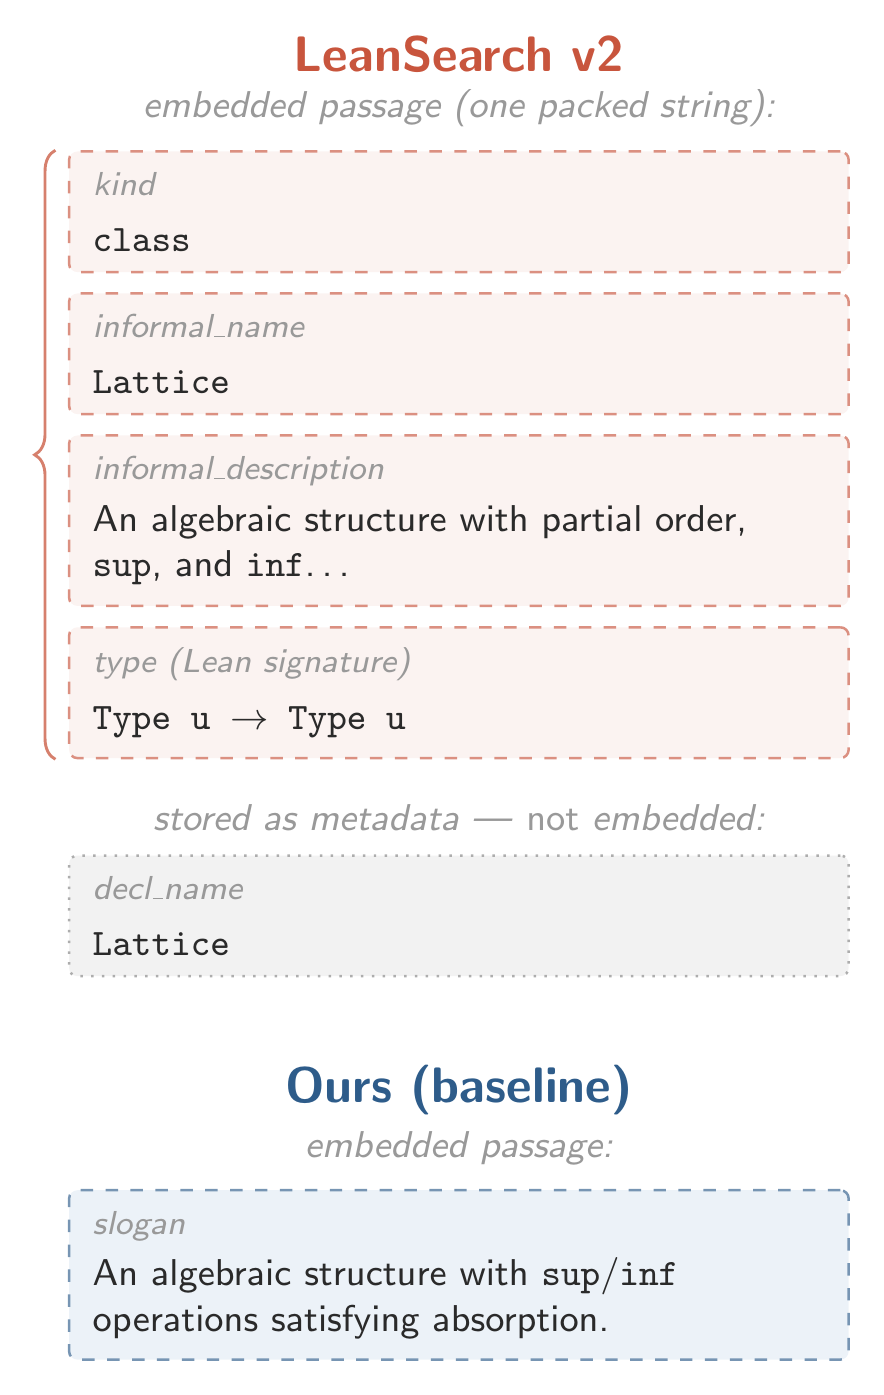
\includegraphics[width=0.25\textwidth]{lsv2_repr_gap_stacked-render-1.png}
    \caption{What each system embeds for a declaration (example: the \texttt{Lattice} class). LeanSearch v2 packs declaration kind, informal name and description, and type signature into a single embedded passage, plus the value body for definitions, classes, and instances. The fully-qualified name is kept only as metadata, outside the embedded text~\cite{leansearch-v2}. Our baseline embeds a single natural-language slogan, with neither the signature nor a lexical handle on the name. The name-and-signature representation and name-matching index we introduce below add that channel.}
    \label{fig:lsv2-repr-gap}
\end{figure}

\paragraph{Closing the gap.}
We group the interventions by what each improves, the ablation in Table~\ref{tab:lsv2_ablation} adds them cumulatively across Configurations A-E.

\begin{itemize}
    \item \textbf{Putting the name where queries can reach it} (\emph{Name/sig}; the name-matching index is part of \emph{Search}). We add a name-and-signature representation: a second embedded passage encoding the declaration's name, type signature, and dependencies. This moves the fully-qualified name, which LSv2 keeps only as metadata, into the embedded text itself (Figure~\ref{fig:lsv2-repr-gap}), giving name-like queries an explicit target. We also add a name-matching index over declaration names for the bare-name queries the embedding may miss. Together these directly fix the two error classes from the representation gap.
    \item \textbf{Translating the query into our wording} (\emph{Search}). For queries written tersely or in Lean syntax, which are unlike our slogans, we have a model draft a hypothetical informal statement answering it and search with that alongside the original query. This fuses the two rankings (HyDE), and phrases the search closer to our slogans.
    \item \textbf{Resolving same-name collisions} (\emph{Graph}). After retrieving, we follow the dependency graph one hop up and add each result's parent declarations (Figure~\ref{fig:graph-expansion}), which surfaces the general concept when a more specific declaration of the same name has outranked it. LSv2 builds the same graph and uses it to inform corpus construction, but does not consult it at retrieval time.
    \item \textbf{Keeping good candidates in the running} (\emph{Search}). We widen the binary-HNSW shortlist (\texttt{ann\_k}) so correct declarations survive into the full-precision cosine pass rather than being pruned early.
\end{itemize}

\begin{figure}[h!]
    \centering
    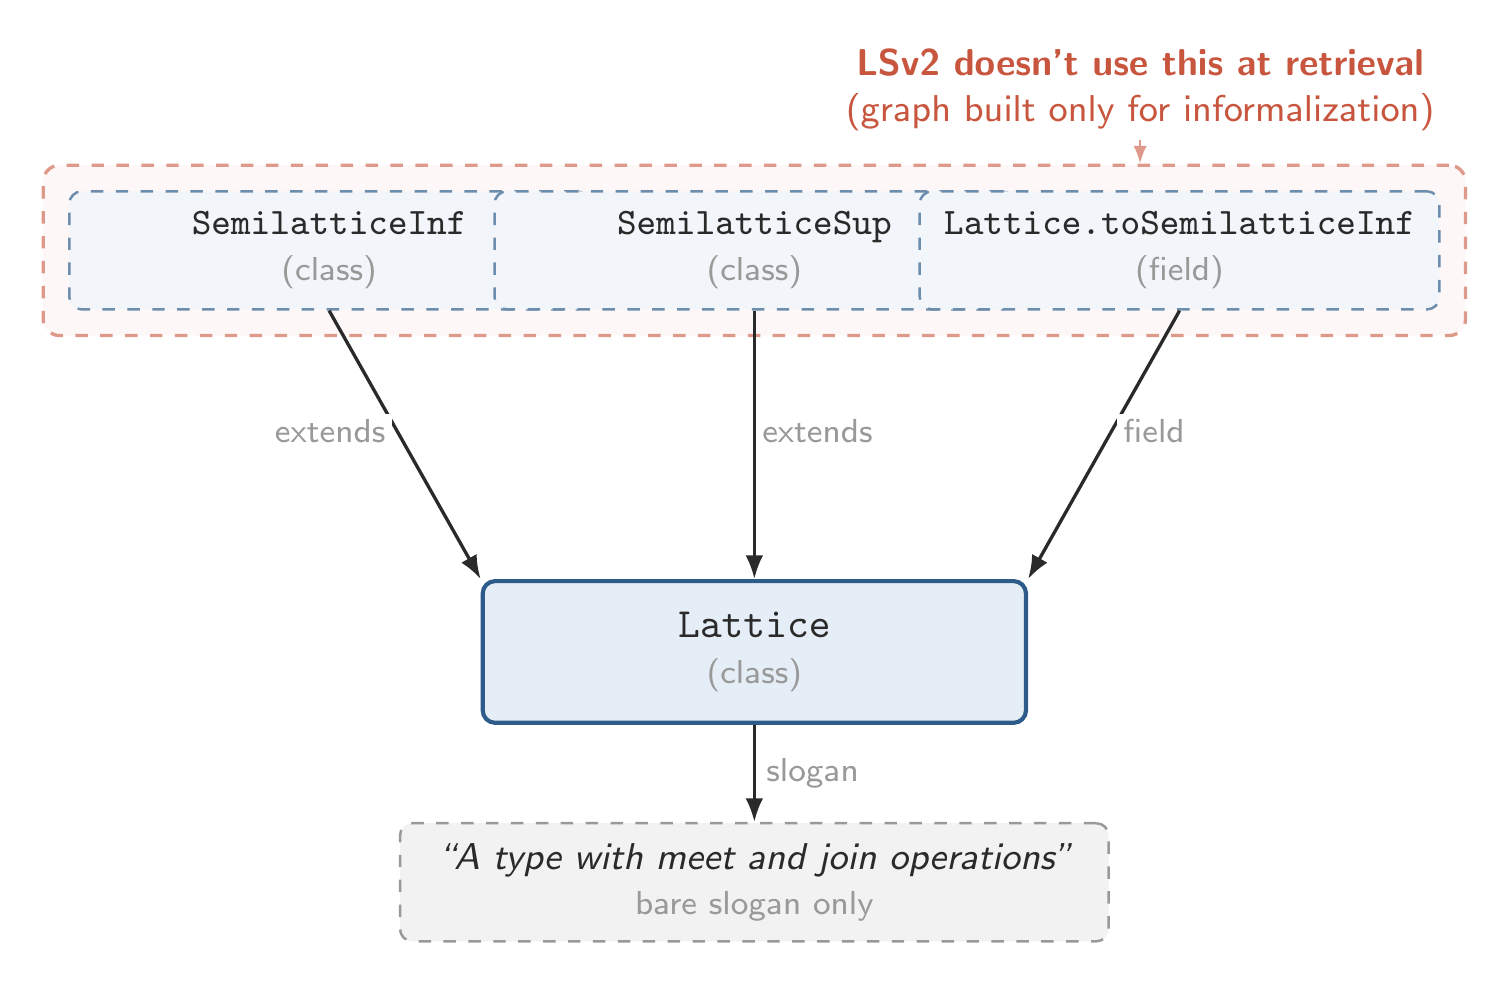
\includegraphics[width=\linewidth]{graph_expansion-render-1.png}
    \caption{Graph expansion on \texttt{Lattice} (Config~E). After retrieval we follow the dependency graph one hop up and add each candidate's \texttt{formal\_dependency} parents. Their names (\texttt{SemilatticeInf}, \texttt{SemilatticeSup}, \texttt{Lattice.toSemilatticeInf}) match name-like queries the bare slogan misses. LSv2 builds the same graph but uses it only for informalization, not at retrieval.}
  \label{fig:graph-expansion}
\end{figure}

\begin{table*}[t]
  \centering \small \setlength{\tabcolsep}{5pt}
  \caption{MathlibQR fair-810. Component columns show what each of our
  configurations uses: the informal slogan, the name-and-signature representation,
  the search-time techniques (name-matching index, query rewriting, wider
  shortlist), and graph expansion. E is recall-optimized, reaching LSv2's reranked
  recall to within 0.5pp (0.775 vs.\ 0.780) without a reranker; F is ranking-optimized.}
  \label{tab:lsv2_ablation}
  \begin{tabular}{l cccc rrrr}
    \toprule
    & \multicolumn{4}{c}{\textbf{Components}} & \multicolumn{4}{c}{\textbf{Metrics}} \\
    \cmidrule(lr){2-5}\cmidrule(lr){6-9}
    \textbf{Configuration} & Slogan & Name/sig & Search & Graph & nDCG@1 & nDCG@5 & nDCG@10 & R@10 \\
    \midrule
    Ours (A) Baseline                    & \checkmark &            &            &            & 0.201 & 0.345 & 0.380 & 0.586 \\
    Ours (B)                             & \checkmark &            & \checkmark &            & 0.262 & 0.441 & 0.467 & 0.680 \\
    Ours (C)                             & \checkmark &            & \checkmark & \checkmark & 0.319 & 0.461 & 0.504 & 0.716 \\
    Ours (D)                             & \checkmark & \checkmark & \checkmark &            & 0.343 & 0.516 & 0.550 & 0.767 \\
    \textbf{Ours (E)} \emph{recall-optimized}  & \checkmark & \checkmark & \checkmark & \checkmark & 0.349 & 0.504 & 0.548 & 0.775 \\
    \midrule
    \textbf{Ours (F)} \emph{ranking-optimized} &            & \checkmark & \checkmark &            & 0.391 & 0.534 & 0.558 & 0.733 \\
    \midrule
    \multicolumn{5}{l}{LSv2 Retriever}            & 0.340 & 0.472 & 0.494 & 0.657 \\
    \multicolumn{5}{l}{LSv2 Retriever + reranker} & \textbf{0.470} & \textbf{0.601} & \textbf{0.623} & \textbf{0.780} \\
    \bottomrule
  \end{tabular}
\end{table*}

\paragraph{Results}
The full ablation is in Table~\ref{tab:lsv2_ablation}; two configurations are worth highlighting. \emph{Ranking-optimized} Configuration~F replaces the slogan with the name-and-signature representation, keeping the search techniques (name-matching index, query rewriting, wider shortlist) but no graph. Without a reranker, it beats LSv2's retriever-only baseline on every metric we report, reaching \textbf{0.558} nDCG@10 against their 0.494 and \textbf{0.733} Recall@10 against their 0.657. Since B and F share the same search techniques and differ only in what they embed, this swap isolates the representation, rather than the search techniques, as the driver of ranking quality.

Combining the slogan with the name-and-signature representation (Configuration~D) and then adding graph expansion (Configuration~E) trades ranking for recall: Recall@10 climbs from 0.733 (F) to 0.767 (D) to \textbf{0.775} (E), while nDCG@10 slips from 0.558 (F) to 0.550 (D) to 0.548 (E). The recall-optimized configuration, E, comes within 0.5pp of LSv2's reranked recall (0.775 vs.\ 0.780) without a reranker;\footnote{Bootstrap 95\% CIs (5000 resamples): Configuration~E Recall@10 0.775~[0.746, 0.802], so LSv2's 0.780 lies within the interval (a failure to reject, not an equivalence test); gains over baseline \mbox{+18.9pp} Recall@10~[+15.1, +22.7] and \mbox{+16.8pp} nDCG@10~[+13.3, +20.2].} neither E nor F matches the reranked nDCG of 0.623, where the reranker's precise ordering leads at every cutoff.

Per declaration type (Figure~\ref{fig:lsv2-perkind}), the levers primarily improve the categories for which slogans were least effective. Structures, classes, definitions, and inductives all benefit, whereas \texttt{theorem} and \texttt{instance}, which typically already have descriptive slogans, decline slightly. Thus, the interventions incur a small cost on well-described declarations in exchange for substantial gains on declarations identified mainly by name. 

\begin{figure*}
    \centering
    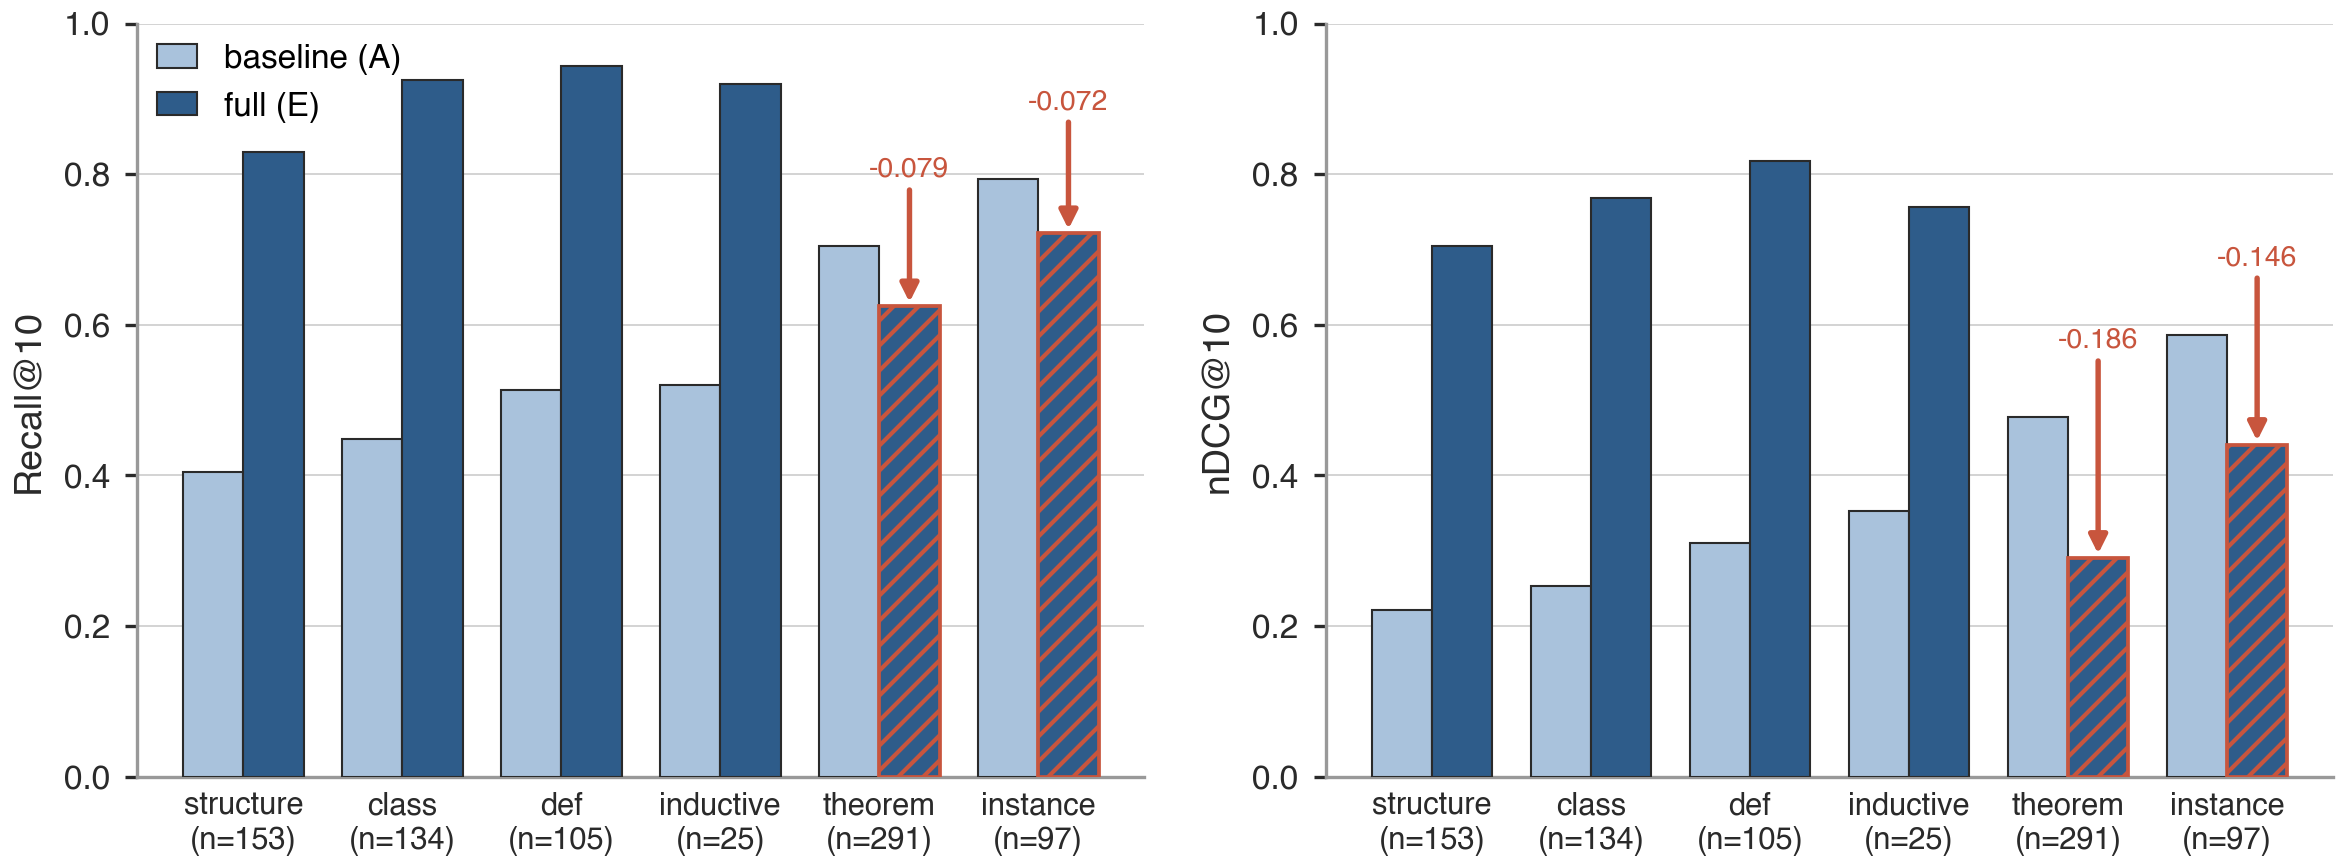
\includegraphics[width=\linewidth]{lsv2_perkind.png}
    \caption{MathlibQR fair-810, Recall@10 by declaration kind, comparing the baseline (Config~A) with the full lever stack (Config~E). The interventions concentrate their gains on declarations identified mainly by name (structures, classes, definitions, and inductives), while \texttt{theorem} and \texttt{instance}, which usually already carry descriptive slogans, decline slightly. Configurations are defined in Table~\ref{tab:lsv2_ablation}.}
    \label{fig:lsv2-perkind}
\end{figure*}

Across the same 810 queries the interventions add \textbf{+18.9pp} Recall@10 and \textbf{+16.8pp} nDCG@10 over the baseline, while graph expansion contributes least once the representation is present (E vs.\ D: +0.8pp Recall, $-$0.2pp nDCG).

% does it transfer to their other benchmarks?
\paragraph{Transfer to MathlibMPR.}
The same configuration does not carry over to chained-premise retrieval. On MathlibMPR, applying the QR-tuned configuration lowers our group Recall@10 from 0.224 to 0.165 against our untuned baseline, so the interventions that help concept retrieval are counterproductive here. The task asks which lemmas a proof invokes, and those can share no vocabulary with the theorem, whereas every technique above sharpens matching on the meaning of a single declaration. We treat this as a scope boundary, not a comparison, and leave chained-premise retrieval to future work.